\documentclass[12pt]{article}

\usepackage[utf8]{inputenc}
\usepackage{latexsym,amsfonts,amssymb,amsthm,amsmath}
\usepackage{tikz}
\usepackage{stanli}
\usetikzlibrary{shapes,calc,through,3d,patterns}
\usetikzlibrary{arrows.meta,decorations.pathreplacing,angles,quotes}
\usepackage{multicol}
\usepackage{geometry}
\usepackage{mathtools}
\usepackage{siunitx}
\usepackage{booktabs}

\setlength{\parindent}{0in}
\setlength{\oddsidemargin}{-0.25in}
\setlength{\textwidth}{7in}
\setlength{\textheight}{9.3in}
\setlength{\topmargin}{-1in}
\setlength{\headheight}{18pt}

\newcommand\blfootnote[1]{%
    \begingroup
    \renewcommand\thefootnote{}\footnote{#1}%
    \addtocounter{footnote}{-1}%
    \endgroup
}

\definecolor{darkred}{rgb}{0.6,0,0}

\newcommand{\bolddelta}{\boldsymbol\delta}
\newcommand{\boldxi}{\boldsymbol\xi}

\begin{document}

\noindent ME473 - Dynamic finite element analysis of structures\hfill EPFL\\
Stefano Burzio \hfill 2025\\
\vspace{0.3cm}

\hspace*{\fill}\textbf{\Large Problem set 6}\hspace*{\fill}

\hrulefill

\subsection*{Problem 1}
Consider a simply supported Euler-Bernoulli beam of length \( \ell \), subject to a downward point load \( P \) applied at the midpoint \( x = \ell/2 \). The beam has constant flexural rigidity \( EI \), cross-sectional area $A$, and density $\rho$.
\begin{center}
    \begin{tikzpicture}[scale=0.8]
        \point{a}{0}{0};
        \point{b}{8}{0};
        \support {1}{a}[0];
        \support {2}{b}[0];
        \draw [thick] (9.70,-0.55) circle [radius=0.05];
        \draw [thick] (10.00,-0.55) circle [radius=0.05];
        \draw [thick] (10.30,-0.55) circle [radius=0.05];
        % Draw the rectangle
        \filldraw[fill=gray!60, draw=black,thick] (0,0) rectangle (10,0.5);
        %axis
        \draw[-latex, ultra thin] (0,0.25) -- (11,0.25);
        \draw[-latex, ultra thin] (0,0) -- (0,2);
        \node at (11.3,0.25) {\(x\)};
        \node at (0,2.2) {\(y\)};
        % length
        \draw[ultra thin] (10,0) -- (10, 2) ;
        \draw[latex-latex, ultra thin]  (0,1)  to node[sloped,midway,above] {$\ell/2$}(5,1) ;
        \draw[latex-latex, ultra thin]  (5,1)  to node[sloped,midway,above] {$\ell/2$}(10,1) ;
        % N
        \draw[-latex, ultra thick] (5,2.5) -- (5,0.5) node[midway, above right]{$P$};
        \draw[ultra thin]  (4,0.3) -- (5,-1) node[right]{$E,A,\rho,I$};
    \end{tikzpicture}
\end{center}
The governing strong form of the beam equation is:
\[
    EI \frac{\partial^4 u_2}{\partial x^4} + \rho A\ddot u_{2}= 0, \quad \text{for } x \in ]0, \ell[
\]
coupled with boundary conditions:
\begin{align*}
     & u_2(0,t) = 0,                                 & \quad u_2(\ell,t) = 0,                                 & \quad \text{\emph{(zero transversal displacement)}}, \\
     & \frac{\partial^2 u_2}{\partial x^2}(0,t) = 0, & \quad \frac{\partial^2 u_2}{\partial x^2}(\ell,t) = 0, & \quad \text{\emph{(zero bending moment)}}            \\
\end{align*}
and the continuity condition:
\[
    \lim_{x\to\ell/2^-} \frac{\partial}{\partial x}\left(-EI\frac{\partial^2u_2}{\partial x^2}\right)-\lim_{x\to\ell/2^+} \frac{\partial}{\partial x}\left(-EI\frac{\partial^2u_2}{\partial x^2}\right)=-P, \qquad \text{\emph{(applied load)}}
\]
\begin{enumerate}
    \item Derive the weak form of the problem by multiplying the equation by a suitable function and integrating by parts to reduce the order of derivatives on $u_2$. Clearly state the function spaces for \( u_2 \) and \( \delta u_2\).
    \item Assuming a finite-dimensional approximation in one beam element
          $$u^h_2(x,t) = \sum_{j=1}^4 h_j(x) q_j(t)$$
          derive the semi-discrete system of equations
          $$\mathbf{K} \mathbf q+\mathbf{M}\ddot{\mathbf q} = \mathbf{r}.$$
          Clearly define the stiffness matrix \( \mathbf{K} \), the mass matrix \( \mathbf{M} \),  and load vector \( \mathbf{r} \).
\end{enumerate}



\subsection*{Problem 2}
Consider the same simply supported Euler-Bernoulli beam, as in the previous problem, of length \( \ell \) with uniform properties \( E, I, A, \rho \), and a point load \( P \) applied at mid-span.

Use the one-element Hermite shape functions and the results for the element stiffness and mass matrices presented in the course to construct and solve the discrete model for the beam. Using the boundary conditions for a simply supported beam, identify the constrained and free degrees of freedom. Reduce the global system by eliminating constrained DOFs.

\begin{enumerate}
    \item Solve the reduced system for the static case (i.e., neglect inertia) and compute the displacement in the middle of the beam due to the point load \( P \). Compare the approximate deflection at mid-span obtained from the exact analytical solution:
          \[
              \delta^\text{exact}=u_2^\text{exact}(\ell/2) = \frac{P \ell^3}{48 EI}.
          \]
          Discuss the relative error and the limitations of using a single finite element.

    \item Use the reduced mass and stiffness matrices to compute the first natural frequency of the beam. Compare your result with the exact fundamental frequency for a simply supported Euler-Bernoulli beam, which is given by:
          \[
              f_1^\text{exact} = \frac{1}{2\pi} \left(\frac{\pi^2}{\ell^2}\right) \sqrt{\frac{EI}{\rho A}}.
          \]
          Discuss and quantify the difference between the computed and exact frequencies. Comment on the accuracy of using a single Hermite element in this case.
\end{enumerate}


\end{document}